%\item Interpretation of results
Although the results described above do not present clear evidence that the Reggio Approach is an effective early childhood program, there are some patterns that emerge and interesting results. 

% summary of main results 

We consider the possibility that it is possible that over time, the programs grew to share more features. Under this scenario, the Reggio Approach and the alternatives would become more similar reducing the estimated treatment effects of the Reggio Approach.\footnote{See \citet{Elango_Hojman_etal_2016_Early-Edu} for a discussion of considering the counterfactual in early childhood education evaluations.} 

There is evidence of policies mandating the provision of early childhood education and encouraging certain guidelines with the aim of improving quality.\footnote{See Appendix~\ref{sec:eceexperiences} for a detailed discussion of these policies.} However, exact information on the trajectory of the systems attended by the individuals in our sample is not published to the best of the authors' knowledge. In order to understand the exact evolution of the programs' administrative and pedagogical components over time, we wrote a survey to structure interviews with key individuals in the different school systems of Reggio Emilia, Parma, and Padova (see Appendix~\ref{sec:survey} for a full description of the survey and its implementation). We asked if the schools had aspects that are also present in the Reggio Approach schools, as well as details about their specific programs. These key aspects that make up the Reggio Approach were collected from published materials as well as confirmed by staff of the Reggio Approach. 

We present the similarities and differences between the different programs in Figures~\ref{fig:agg-admin} and~\ref{fig:agg-ped}. Using results from the structured interviews, we compute the number of administrative and pedagogical components that each program shares with the Reggio Approach by school type, city, and year. We examine 14 administrative components and 12 pedagogical components. Over time, many of the programs other than the state programs, adopt more features present in the Reggio Approach. This is especially true of the Parma municipal program when examining administrative components. The other programs do not adopt as many pedagogical components as they do administrative ones. Even though the Reggio Approach remained distinctive when considering the sum of its elements, many of the alternative schools evolved to include certain elements.

\begin{figure}[H]
\begin{center}
\begin{subfigure}[b]{0.55\textwidth}
	\caption{Number of Administrative Characteristics in Common with the Reggio Approach}\label{fig:agg-admin}
	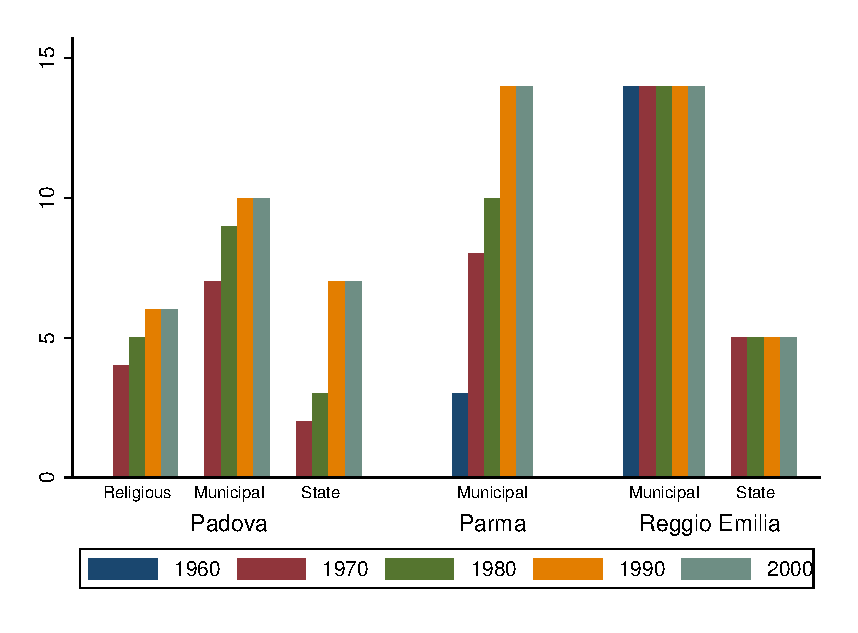
\includegraphics[width=\textwidth]{../../output/aggregateAdministrative.eps}
\end{subfigure}%
~
\begin{subfigure}[b]{0.55\textwidth}
	\caption{Number of Pedagogical Characteristics in Common with the Reggio Approach}\label{fig:agg-ped}
	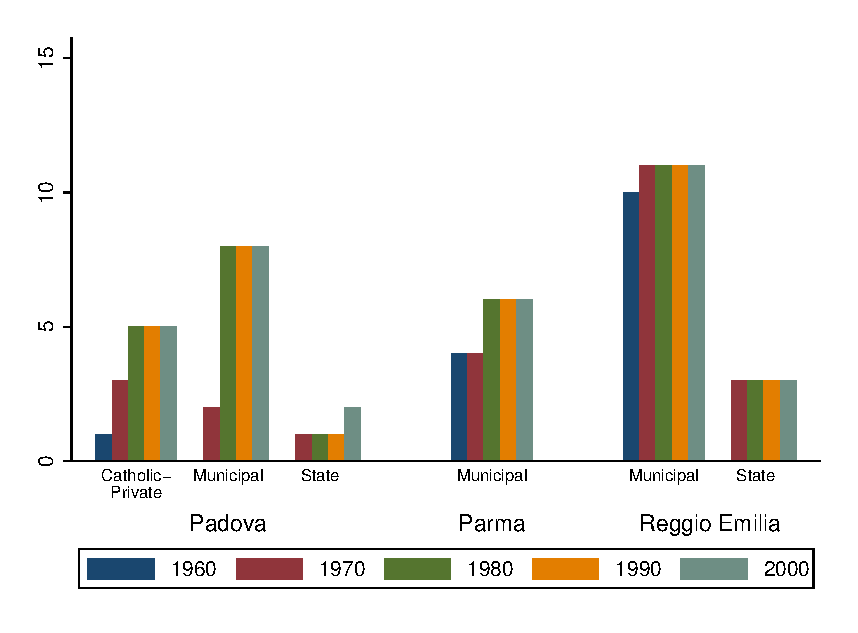
\includegraphics[width=\textwidth]{../../output/aggregatePedagogical.eps}
\end{subfigure}%
\end{center}
\raggedright \footnotesize Note: These graphs show the number of administrative and pedagogical components that each program has in common with the Reggio Approach. We consider 14 administrative components and 12 pedagogical components. Some of the pedagogical components were not present in the Reggio Approach. 
\end{figure}

See Appendix~\ref{sec:survey} for a more detailed description of the survey results. We highlight the items that are related to prioritizing disadvantaged children. Municipal schools in the three cities shared priorities of enrolling economically disadvantaged children, children from a single-parent household, and children with disabilities. This is seen in our results given that controlling for more background characteristics makes the results more positive when comparing those who attended the Reggio Approach to other individuals in Reggio Emilia. These results are also similar in magnitude, and for adolescents and children similar in significance, to the AIPW results. Given that AIPW is an estimator that can help correct bias from poor model specification, the similarity of estimates highlight that the background variables balance the sample between those who selected into the Reggio Approach and those who did not. 

In addition to this historical context, we expand on shortcomings in the data that make more precise analysis difficult. We presented estimates with different control sets to better understand the importance of observed background characteristics that can determine this selection. With more precise background variables, such as a more complete variable for family income, we could better capture the disadvantage in the sample, allowing our estimates to be less biased. More background variables for the older cohorts would be especially useful considering there were fewer available for them.

Another data shortcoming occurs in the outcomes. Although the survey was designed to capture a rich set of variables from life-relevant 


